\section*{Exercise 3}

\subsection*{Exercise 3 (2)}
Explain why (in terms of the evaluation process) these two programs give different answers 
(i.e. have different distributions on return values):
\begin{lstlisting}
(define foo (flip))
(list foo foo foo)
\end{lstlisting}

\begin{lstlisting}
(define (foo) (flip))
(list (foo) (foo) (foo))
\end{lstlisting}    

\paragraph{Solution} 
In the first program \texttt{foo} is defined as a variable and the value of the evaluation of the expression \texttt{(flip)} is
assigned to it; indeed, the value of \texttt{foo} is either \texttt{\#t} or \texttt{\#f}.
After that a list is created which contains three time the value assigned to the variable \texttt{foo}, so if \texttt{foo} has value
\texttt{\#t}, then the list is defined as follows: \texttt{\textquotesingle(\#t \#t \#t)}; otherwise the created list is:
\texttt{\textquotesingle(\#f \#f \#f)}.

In the second program, we a new procedure called \texttt{foo} is defined which is a wrapper for the \texttt{flip} procedure. This means
that whenever the procedure \texttt{foo} is called, also \texttt{flip} is called.
Therefore, when defining the list, the expression \texttt{flip} is evaluated three times and, since it is a non-deterministic 
procedure, the three elements of the list can be different.


\subsection*{Exercise 3 (5)}
Here is a modified version of the tug of war game. Instead of drawing strength from the continuous Gaussian 
distribution, strength is either 5 or 10 with equal probability. Also the probability of laziness is changed from 1/4 to 1/3. 
Here are four expressions you could evaluate using this modified model:

\begin{lstlisting}
(define strength (mem (lambda (person) (if (flip) 5 10))))
(define lazy (lambda (person) (flip (/ 1 3))))
    
(define (total-pulling team)
  (sum
   (map (lambda (person) (if (lazy person)
                             (/ (strength person) 2)
                             (strength person)))
        team)))
    
(define (winner team1 team2)
  (if (< (total-pulling team1) (total-pulling team2))
      team2
      team1))
    
(winner '(alice) '(bob))                        ;; expression 1
    
(equal? '(alice) (winner '(alice) '(bob)))      ;; expression 2
    
(and (equal? '(alice) (winner '(alice) '(bob))) ;; expression 3
     (equal? '(alice) (winner '(alice) '(fred))))
    
(and (equal? '(alice) (winner '(alice) '(bob))) ;; expression 4
     (equal? '(jane) (winner '(jane) '(fred))))
\end{lstlisting}

\begin{itemize}
    \item[a.] Write down the sequence of expression evaluations and random choices that will be made in evaluating each expression.
    \item[b.] Directly compute the probability for each possible return value from each expression.
    \item[c.] Why are the probabilities different for the last two? Explain both in terms of the probability calculations 
        you did and in terms of the “causal” process of evaluating and making random choices.
\end{itemize}

\paragraph{Solution}
\begin{itemize}
    \item[a.] First of all, the procedures are defined and the interpreter associates the name of the procedures with their definition
        in the \textit{global environment}.
        Then the interpreter evaluates the four expressions in the order in which they are written: 
        
        \paragraph*{Expression 1} \texttt{(winner \textquotesingle(alice) \textquotesingle(bob))} 
        
        The first step is to retrieve the body of the procedure \texttt{winner}. Then the formal parameters are substituted by 
        the actual parameters \texttt{\textquotesingle(alice)} and \texttt{\textquotesingle(bob)}. 
        Now the interpreter has to evaluate the following expression:
        \begin{lstlisting}[caption={Body of procedure \texttt{winner} with actual parameters}, captionpos=b]
(if (< (total-pulling '(alice)) (total-pulling '(bob)))
    '(bob)
    '(alice))
        \end{lstlisting}
        The following step is to evaluate the conditional expression, so it starts by evaluating the \textit{predicate}: 
        \texttt{(< (total-pulling \textquotesingle(alice)) (total-pulling \textquotesingle(bob)))}. 
        The interpreter has to deal with the primitive predicate ``\texttt{<}'', so it has to evaluate the arguments and then 
        it has to apply the predicate to the evaluated arguments.
        The first argument to evaluate is \texttt{(total-pulling \textquotesingle(alice))}: the body of the \texttt{total-pulling} procedure 
        is retrieved in the \textit{global environment} and the expression is substituted by the body of the procedure.
        Afterwards the actual parameter is applied to the body of the procedure and the expression 
        \texttt{(total-pulling \textquotesingle(alice))} becomes as follows:
        \begin{lstlisting}[caption={Body of procedure \texttt{total-pulling} with actual parameters \texttt{\textquotesingle(alice)}}, captionpos=b, label={lst:t-p}]
(sum
 (map (lambda (person) (if (lazy person)
                           (/ (strength person) 2)
                           (strength person)))
      '(alice)))
        \end{lstlisting}
        The procedure \texttt{sum} takes as argument a list of numbers and returns the sum over the elements of the list. In this case
        the argument of the procedure is another expression, so the interpreter has to evaluateit and then apply it to the \texttt{sum}
        procedure.
        Now the expression to be evaluated is the following:
        \begin{lstlisting}[caption={Argument of procedure \texttt{sum} in Listing~\ref{lst:t-p}}, captionpos=b, label={lst:map}]
(map (lambda (person) (if (lazy person)
                          (/ (strength person) 2)
                          (strength person)))
     '(alice))
        \end{lstlisting}
        The \texttt{map} procedure takes as arguments a \textit{lambda} expression and a list. The procedure applies the
        \textit{lambda} expression to each element of the list and returns the list of the results of the \textit{lambda}
        expression on the elements of the list in input.
        So the first step consists of evaluating the \textit{lambda} expression with argument \texttt{\textquotesingle alice}. 
        The resulting expression is the body of the \textit{lambda} expression with the formal parameter \texttt{person} substituted 
        by the actual parameter \texttt{\textquotesingle alice}:
        \begin{lstlisting}[caption={Application of \texttt{map} prcedure of Listing~\ref{lst:map}}, 
            captionpos=b, label={lst:lambda-body}]
(if (lazy 'alice) (/ (strength 'alice) 2) (strength 'alice))
        \end{lstlisting}
        Since the interpreter has to evaluate a conditional expression, the interpreter firsts evaluate the \textit{predicate}.
        To evaluate the call \texttt{(lazy \textquotesingle alice)}, the interpreter first takes the body of the procedure and then substitutes
        all the occurences of formal parameter by the value of the actual parameter. The resulting expression is:
        \begin{lstlisting}[caption={Body of procedure \texttt{lazy} when evaluating Listing~\ref{lst:lambda-body}}, captionpos=b]
(flip (/ 1 3))
        \end{lstlisting}
        The procedure \texttt{flip} is a probabilistic procedure, it can take as parameter the probability to return \texttt{\#t}.
        In our case, the interpreter has to evaluate the expression \texttt{(/ 1 3)} and than apply the result to the procedure 
        \texttt{flip}.
        We suppose that the result of the call \texttt{(flip 1/3)} is \texttt{\#f}, so the result of the evaluation of the
        \textit{predicate} in the conditional expression is \texttt{\#f}. Since the \textit{predicate} is false, the interpreter has
        to evaluate the \textit{alternative} expression \texttt{(strength \textquotesingle alice)}.
        It is a procedure call, so the interpreter has to retrieve the body of the procedure and then substitute the formal
        parameter by the actual one.
        The result is that the interpreter now has to evaluate the following expression:
        \begin{lstlisting}[caption={Body of procedure \texttt{strength} when evaluating Listing~\ref{lst:lambda-body}}, captionpos=b]
(if (flip) 5 10)
        \end{lstlisting}
        The \texttt{strength} procedure is a particular type of procedure, indeed, it is memoized through the \texttt{mem} procedure.
        This means that the first time the procedure is called, the result of the call is memorized and each time the procedure is
        called with the same argument, the interpreter does not evaluate the function, but it retireves the already computed
        result in the \textit{global environment}. This is the first time that \texttt{(strength \textquotesingle alice)} is evaluated, 
        so the procedure has to be evaluated in a ``standard'' way.
        The body of the procedure is composed by a conditional expression, the \texttt{flip} procedure is evaluated and we suppose
        that the result is \texttt{\#t}, so the procedure \texttt{strength} returns the value $5$.

        Thus, the expression \texttt{(strength \textquotesingle alice)} is evaluated with $5$; since the second argument of the \texttt{map} procedure
        is a list with only one argument (i.e. \texttt{\textquotesingle alice}) the result is a list with only one element (i.e. $5$).
        This list is the argument of the procedure \texttt{sum} and the interpreter has to evaluate the following expression:
        \begin{lstlisting}[caption={Expression to be evaluated after evaluating the expression in Listing~\ref{lst:map}}, captionpos=b]
(sum '(5))
        \end{lstlisting}
        Which is evaluated with $5$. This is the result of the evaluation of the call \texttt{(total-pulling \textquotesingle (alice))}, now the
        interpreter has to evaluate the second argument of the expression \texttt{(< 5 (total-pulling \textquotesingle (bob)))}, since $5$ is 
        a primitive expression and it cannot be reduced anymore.
        The evaluation of the expression \texttt{(total-pulling \textquotesingle (bob))} is the same as the expression 
        \texttt{(total-pulling \textquotesingle (alice))}, but, since there are some probabilistic cases, the result can be different. In particular,
        we suppose that the evaluation of \texttt{(lazy \textquotesingle bob)} returns the value \texttt{\#t}, so the interpreter has to evaluate the
        expression \texttt{(/ (strength \textquotesingle bob) 2)} instead of \texttt{(strength \textquotesingle bob)}. The interpreter has to evaluate a primitive
        procedure, thus it has to evaluate first the operands and then to apply the operator to them.
        We suppose that the evaluation of \texttt{(strength \textquotesingle bob)} returns the value $5$. It is important to notice that it is the
        first time that the \texttt{strength} procedure is called with actual parameter \texttt{\textquotesingle bob}, so the evaluation is
        ``standard'' and the result of the call is memorized in the \textit{global environment}. 
        Therefore the expression \texttt{(/ (strength \textquotesingle bob) 2)} is evaluated with $2.5$.

        Now the situation is represented in the following way:
        \begin{lstlisting}[caption={Expression to be evaluated after evaluating \texttt{(total-pulling \textquotesingle bob)}}, captionpos=b]
(if (< 5 2.5)
    '(bob)
    '(alice)))  
        \end{lstlisting}
        Since $5 > 2.5$, the \textit{predicate} is false and the value \texttt{\textquotesingle(alice)} is returned. Thus the \textit{expression 1}
        is evaluated with the value \texttt{\textquotesingle(alice)}.


        \paragraph*{Expression 2} \texttt{(equal? \textquotesingle(alice) (winner \textquotesingle(alice) \textquotesingle(bob)))}

        The predicate \texttt{equal?} returns \texttt{\#t} when the two arguments are euqal, it returns \texttt{\#f} otherwise, so
        the interpreter has to evaluate the two \textit{operands} and then to compare them. The first \textit{operand} is a quoted
        data object, so it is a list which contains the symbol \texttt{\textquotesingle alice}. The evaluation of the second \textit{operand} is
        identical to the evaluation of \textit{expression 1}.
        
        Since there are some probabilistic procedures which have to be evaluated, the result of the evaluation could be different 
        from the previous one. In particular we suppose that in this case the call \texttt{(lazy \textquotesingle alice)} returns \texttt{\#f} and 
        the call \texttt{(lazy \textquotesingle bob)} returns \texttt{\#f}.
        Since the \texttt{strength} procedure is memoized, the calls \texttt{(strength \textquotesingle alice)} and \texttt{(strength \textquotesingle bob)} return
        the same values as before, i.e. both the calls return the value $5$.
        
        The two teams \texttt{\textquotesingle(alice)} and \texttt{\textquotesingle(bob)} have the same strength (i.e $5$), 
        therefore the evaluation of the \texttt{winner} procedure returns \texttt{\textquotesingle (alice)}.
        Given that the two arguments of the predicate \texttt{equal?} are equal, the evaluation of \textit{expression 2} is \texttt{\#t}.


        \paragraph*{Expression 3} The \textit{expression 3} is the following one: 
        \begin{lstlisting}
(and (equal? '(alice) (winner '(alice) '(bob)))
     (equal? '(alice) (winner '(alice) '(fred))))
        \end{lstlisting}

        The logical composition \texttt{and} is evaluated by first evaluating the first operand.
        If the evaluation returns \texttt{\#t}, then the second operand is evaluated; if it is \texttt{\#t}, then is evaluated the 
        third one (if present) and so on and so forth.
        If all the values of the operands are \texttt{\#t}, then the evaluation of the expression is \texttt{\#t}, otherwise when
        one operand is evaluated as \texttt{\#f}, the expression is evaluated as \texttt{\#f} and the follwing operands are not
        evaluated.
        
        So the interpreter evaluates the first \texttt{equal?} expression and the evaluation is the same as the previous case.
        We suppose now that \texttt{\textquotesingle alice} is \textit{lazy} and \texttt{\textquotesingle bob} is not \textit{lazy}.
        In this case the \texttt{winner} procedure returns the value \texttt{\textquotesingle (bob)}, so the evaluation of the first 
        operand returns the value \texttt{\#f}.
        Thus the evaluation of the \texttt{and} is stopped and the returned value is \texttt{\#f}.


        \paragraph*{Expression 4} The \textit{expression 4} is the following one: 
        \begin{lstlisting}
(and (equal? '(alice) (winner '(alice) '(bob)))
     (equal? '(jane) (winner '(jane) '(fred))))
        \end{lstlisting}

        We have already dissussed in detail about the evaluation of the procedures and predicates in this expression, so the main
        argumentation concerns the results of the evaluation of the \textit{expression 4}.
        Let us suppose that \texttt{\textquotesingle alice} is not \textit{lazy} and \texttt{\textquotesingle bob} is \textit{lazy}. 
        The first argument of the \texttt{and} predicate is \textit{true}, so the interpreter has to evaluate the second expression.
        
        Since both the calls \texttt{(strength \textquotesingle jane)} and \texttt{(strength \textquotesingle fred)} have never been evaluated, 
        their evaluation happens in a ``standard'' way and their values are memorized into the \textit{global environment}.
        Let us suppose both \texttt{\textquotesingle jane} and \texttt{\textquotesingle fred} are strong, so the value returned by the procedure \texttt{strength}
        is $10$. Now let us suppose that the evaluation of \texttt{(lazy \textquotesingle jane)} is \texttt{\#f} and the evaluation of 
        \texttt{(lazy \textquotesingle fred)} is \textit{ture}.

        Therefore the evaluation of \texttt{(winner \textquotesingle(jane) \textquotesingle(fred))} returns \texttt{\textquotesingle(jane)} 
        which makes \textit{true} the second expression \texttt{equal?}. 
        Since both the operands of the \texttt{and} predicate are \textit{true}, the evaluation of the \textit{expression 4} is 
        \texttt{\#t}.

    \item[b.] To compute the probability for each possible return value from each expression it has been decided that the execution
        of the four expressions is sequential. For this reason, it is necessary to make some assumption when the procedure \texttt{strength} is
        called, since it is a memoized procedure. This means that the first evaluation influences the following calls.

        \paragraph*{Expression 1} When the interpreter has to evaluate this first expression, the procedure \texttt{strength} has never 
        called before for both \texttt{\textquotesingle alice} and \texttt{\textquotesingle bob}, so they can assume either the value $5$ or $10$ after evaluating
        the procedure \texttt{strength}. Furthermore they can result either \textit{lazy} or \textit{not lazy}, thus there are
        $16$ combinations of values that the two teams can assume.
        In particular, it is possible to build a table whose rows and columns are composed by all the possible combinations of
        the outcomes of the probabilistic procedures \texttt{strength} and \texttt{lazy}, in particular
        the rows are all the possible outcomes of the evaluations of the procedures for one team (i.e. \texttt{\textquotesingle (alice)}), 
        while the columns are all the possible outcomes of the evaluations of the procedures for the other team (i.e. \texttt{\textquotesingle (bob)}).
        Each cell of the table contains the probability to get that particular case. The computed probability are shown
        in Table~\ref{tab:exp-1}.
        The table shows all the possible combinations of values that \texttt{\textquotesingle alice} and \texttt{\textquotesingle bob} can get, the cells coloured
        in Violet are the cases where \texttt{\textquotesingle alice} wins over \texttt{\textquotesingle bob}, instead, the cells coloured in Orange are those
        where \texttt{\textquotesingle bob} wins.

        Thus to compute the probability that \texttt{\textquotesingle (alice)} wins it is sufficient to sum all the probabilities coloured in Violet,
        while to compute the probability that \texttt{\textquotesingle (bob)} wins it is sufficient to sum all the probabilities coloured in Orange.
        The result is the following:
        \[ P(winner = alice) = 25 / 36 \]
        \[ P(winner = bob) = 11 / 36 \]
        \begin{table}[H]
            \centering
            \bgroup
                \def\arraystretch{1.5}
                \begin{tabular}{| l | C{1.8cm} C{1.8cm} C{1.8cm} C{1.8cm}  |}                    
                    \hline
                    \backslashbox{\textcolor{Violet}{\textbf{\textquotesingle(alice)}}}{\textcolor{RedOrange}{\textbf{\textquotesingle(bob)}}} & 
                        \textbf{strong lazy} & \textbf{strong $\neg$lazy} & \textbf{$\neg$strong lazy} & \textbf{$\neg$strong $\neg$lazy} \\
                    \hline

                    \textbf{strong $\land$ lazy} & \textcolor{Violet}{$1/36$} & \textcolor{RedOrange}{$1/18$} & 
                        \textcolor{Violet}{$1/36$} & \textcolor{Violet}{$1/18$} \\ 

                    \textbf{strong $\land$ $\neg$lazy} & \textcolor{Violet}{$1/18$} & \textcolor{Violet}{$1/9$} & 
                        \textcolor{Violet}{$1/18$} & \textcolor{Violet}{$1/9$} \\ 
                    
                    \textbf{$\neg$strong $\land$ lazy} & \textcolor{RedOrange}{$1/36$} & \textcolor{RedOrange}{$1/18$} & 
                        \textcolor{Violet}{$1/36$} & \textcolor{RedOrange}{$1/18$} \\ 
                    
                    \textbf{$\neg$strong $\land$ $\neg$lazy} & \textcolor{Violet}{$1/18$} & \textcolor{RedOrange}{$1/9$} & 
                        \textcolor{Violet}{$1/18$} & \textcolor{Violet}{$1/9$} \\
                    \hline
                \end{tabular}
            \egroup
            \caption{
                Probabilities of all possible cases of the \textit{expression 1}. The cells coloured in Violet are the ones where
                \texttt{\textquotesingle alice} wins against \texttt{\textquotesingle bob}.
            }
            \label{tab:exp-1}
        \end{table}
     
        \paragraph*{Expression 2} Since the procedure \texttt{strength} is memoized, the results of the evaluation of the previous
        expression influences the the probability for each possible outcome of this expression.
        In particular, the values of the strength of both \texttt{\textquotesingle alice} and \texttt{\textquotesingle bob} are fixed, thus the probabilistic
        behaviour of the evaluation of this expression depends only on the result of the procedure \texttt{lazy}, so the table
        of probabilities has less entries.

        Let us suppose that during the evaluation of the \textit{expression 1} the strength assigned to both \texttt{\textquotesingle alice} and
        \texttt{\textquotesingle bob} is $5$. Thus the table contains only four different cases: \textit{(i)} Both \texttt{\textquotesingle alice} and
        \texttt{\textquotesingle bob} are \textit{lazy}; \textit{(ii)} \texttt{\textquotesingle alice} is \textit{lazy} and \texttt{\textquotesingle bob} is \textit{lazy};
        \textit{(iii)} \texttt{\textquotesingle alice} is \textit{not lazy} and \texttt{\textquotesingle bob} is \textit{lazy}; \textit{(iv)} Both \texttt{\textquotesingle alice} and
        \texttt{\textquotesingle bob} are \textit{not lazy}.
        The Table~\ref{tab:exp-2} represents the different probabilities of all possible cases: also in this case, the cells coloured
        in Violet are the ones where \texttt{\textquotesingle alice} wins. The result is the following:
        \[ P(winner = alice\;|\;strength(alice) = 5 \land strength(bob) = 5) = 7/9 \]
        The probability that the \textit{expression 2} returns the value \texttt{\#t} is $7/9$ and the probability that it
        returns the value \texttt{\#f} is $2/9$.
        \begin{table}[H]
            \centering
            \bgroup
                \def\arraystretch{1.5}
                \begin{tabular}{| c | c c|}                    
                    \hline
                    \backslashbox{\textcolor{Violet}{\textbf{\textquotesingle(alice)}}}{\textcolor{RedOrange}{\textbf{\textquotesingle(bob)}}} & 
                        \textbf{lazy} & \textbf{$\neg$lazy} \\
                    \hline

                    \textbf{lazy} & \textcolor{Violet}{$1/9$} & \textcolor{RedOrange}{$2/9$} \\ 

                    \textbf{$\neg$lazy} & \textcolor{Violet}{$2/9$} & \textcolor{Violet}{$4/9$} \\ 
                    \hline
                \end{tabular}
            \egroup
            \caption{
                Probabilities of all possible cases of the \textit{expression 2}. The cells coloured in Violet are the ones where
                \texttt{\textquotesingle alice} wins against \texttt{\textquotesingle bob}.
                It is important to remeber that both \texttt{\textquotesingle alice} and \texttt{\textquotesingle bob} are \textit{weak} (i.e. the value assigned to
                their strength is $5$).
            }
            \label{tab:exp-2}
        \end{table}

        \paragraph*{Expression 3} This expression contains the logical operator \texttt{and}, so the value returned is \texttt{\#t}
        if both the operands are \textit{true}. The first operand is euqal to the previous expression, while the second operand
        is different: the first team (i.e. \texttt{\textquotesingle (alice)}) has already an assigned value to the \textit{strength}, while the second 
        team (i.e. \texttt{\textquotesingle (fred)}) has not any assigned value to the \textit{strength}.

        It is important to remeber that the second operand is not interpreted if the first one is evaluated as \texttt{\#f}, but this
        fact does not influence the probabilities of the outcomes of this expression, it could affect the probabilities of the
        \textit{expression 4}.

        The expression can be divided in two independent parts: the first one is the match between \texttt{\textquotesingle (alice)} and 
        \texttt{\textquotesingle (bob)} and the second part is the match between \texttt{\textquotesingle (alice)} and \texttt{\textquotesingle (fred)}. 
        Since these two parts are independent, it is possible to compute the probabilities of these parts and then multiply them to
        get the final probability.
        
        The first probability to compute is euqal to the probability of \textit{expression 2}, so we can refer to the 
        Table~\ref{tab:exp-2} and the probability to get the value \textit{true} is $7/9$.
        Regarding the second operand, it is necessary to consider different cases, indeed, the interpreter has to evaluate only the
        laziness of \texttt{\textquotesingle alice} and it has to evaluate both the strength and laziness of \texttt{\textquotesingle fred}. For this reason it is
        possible to compute a table with two rows (i.e. the number possible values of the laziness of \texttt{\textquotesingle alice}) and four columns
        (i.e. the number of possible combinations of the strength and laziness of \texttt{\textquotesingle fred}).
        The Table~\ref{tab:exp-3} contains the probabilities for all possible cases of the second part of the \textit{expression 3}.

        \begin{table}[H]
            \centering
            \bgroup
                \def\arraystretch{1.5}
                \begin{tabular}{| l | C{1.8cm} C{1.8cm} C{1.8cm} C{1.8cm}  |}                    
                    \hline
                    \backslashbox{\textcolor{Violet}{\textbf{\textquotesingle (alice)}}}{\textcolor{RedOrange}{\textbf{\textquotesingle (fred)}}} & 
                        \textbf{strong lazy} & \textbf{strong $\neg$lazy} & \textbf{$\neg$strong lazy} & \textbf{$\neg$strong $\neg$lazy} \\
                    \hline

                    \textbf{$\left(\neg\text{ strong}\right)$ lazy} & \textcolor{RedOrange}{$1/18$} & \textcolor{RedOrange}{$1/9$} & 
                        \textcolor{Violet}{$1/18$} & \textcolor{RedOrange}{$1/9$} \\ 

                    \textbf{$\left(\neg\text{ strong}\right)$ $\neg$lazy} & \textcolor{Violet}{$1/9$} & \textcolor{RedOrange}{$2/9$} & 
                        \textcolor{Violet}{$1/9$} & \textcolor{Violet}{$2/9$} \\

                    \hline
                \end{tabular}
            \egroup
            \caption{
                Probabilities of all possible cases of the second part of the \textit{expression 3}. 
                The cells coloured in Violet are the ones where \texttt{\textquotesingle alice} wins against \texttt{\textquotesingle fred}.
                It is important to remeber that \texttt{\textquotesingle alice} is \textit{weak} (i.e. the value assigned to her strength is $5$).
            }
            \label{tab:exp-3}
        \end{table}

        The result is that the probability that the second part of the expression is evaluated with \textit{true} is $1/2$, indeed,
        it is returned \texttt{\#t} when \texttt{\textquotesingle (alice)} wins against \texttt{\textquotesingle (fred)}. 
        As said before, it is possible to compute the final probability by multipling the probabilities of the two parts. 
        Thus it results that the probability to get the value \texttt{\#t} is
        $7/9\;\cdot\;1/2 = 7/18$. While the probability to get the value \texttt{\#f} is given by 
        $P(outcome = false\;|\;strength(alice) = strength(bob) = 5) = 1 - 7/18 = 11/18$.
        
        \paragraph*{Expression 4} The computation of the probability for each possible result of this expression is strongly 
        influenced by the result of the previous expression, indeed, if the second part of the \textit{expression 3} is evaluated,
        then it is necessary to compute the probability conditioned by the value assigned to the \textit{strength} of \texttt{\textquotesingle fred}.
        Otherwise the probabilities to compute are conditioned only by the values assigned to the \textit{strength} of \texttt{\textquotesingle alice}
        and \texttt{\textquotesingle bob}.

        Let us suppose that the result of the first part of the previous expression is \texttt{\#f}, so the second part has not been
        evaluated and the value of the \textit{strength} of \texttt{\textquotesingle fred} is not fixed.
        The computation of the probabilities for this expression is similar to the previous one, indeed, there are two independent
        parts logically connected by the \texttt{and} predicate. The first part is equal to the \textit{expression 2} 
        (Table~\ref{tab:exp-2}), while the second part is equivalent to the \textit{expression 1}, since both \texttt{\textquotesingle jane} and
        \texttt{\textquotesingle fred} have never been uesd as parameter of the \texttt{strength} procedure.
        The Table~\ref{tab:exp-4} represents all the possible cases of the second part of this expression and it is equal to
        the Table~\ref{tab:exp-1}. The table is shown for greater clearly. 
        \begin{table}[H]
            \centering
            \bgroup
                \def\arraystretch{1.5}
                \begin{tabular}{| l | C{1.8cm} C{1.8cm} C{1.8cm} C{1.8cm}  |}                    
                    \hline
                    \backslashbox{\textcolor{Violet}{\textbf{\textquotesingle (jane)}}}{\textcolor{RedOrange}{\textbf{\textquotesingle (fred)}}} & 
                        \textbf{strong lazy} & \textbf{strong $\neg$lazy} & \textbf{$\neg$strong lazy} & \textbf{$\neg$strong $\neg$lazy} \\
                    \hline

                    \textbf{strong $\land$ lazy} & \textcolor{Violet}{$1/36$} & \textcolor{RedOrange}{$1/18$} & 
                        \textcolor{Violet}{$1/36$} & \textcolor{Violet}{$1/18$} \\ 

                    \textbf{strong $\land$ $\neg$lazy} & \textcolor{Violet}{$1/18$} & \textcolor{Violet}{$1/9$} & 
                        \textcolor{Violet}{$1/18$} & \textcolor{Violet}{$1/9$} \\ 
                    
                    \textbf{$\neg$strong $\land$ lazy} & \textcolor{RedOrange}{$1/36$} & \textcolor{RedOrange}{$1/18$} & 
                        \textcolor{Violet}{$1/36$} & \textcolor{RedOrange}{$1/18$} \\ 
                    
                    \textbf{$\neg$strong $\land$ $\neg$lazy} & \textcolor{Violet}{$1/18$} & \textcolor{RedOrange}{$1/9$} & 
                        \textcolor{Violet}{$1/18$} & \textcolor{Violet}{$1/9$} \\
                    \hline
                \end{tabular}
            \egroup
            \caption{
                Probabilities of all possible cases of the second part of the \textit{expression 4}. 
                The cells coloured in Violet are the ones where \texttt{\textquotesingle jane} wins against \texttt{\textquotesingle fred}.
            }
            \label{tab:exp-4}
        \end{table}

        The result is that the \textit{expression 4} returns the value \texttt{\#t} with probability $7/9 \cdot 25/36 = 175/324 
        \approx 0.54$, while the probability to get the value \texttt{\#f} is $1 - 175/324 = 149/324 \approx 0.46$.

    \item[c.] The computed probabilities of \textit{expression 3} and \textit{expression 4} are different because in the first case
        the strength of three teams is certainly fixed, indeed, the strength of both \texttt{\textquotesingle alice} and \texttt{\textquotesingle bob} is assigned
        during the evaluation of the \textit{expression 1}. Instead, in the second case, the strength is assigned certainly to two
        teams (i.e. \texttt{\textquotesingle (alice)} and \texttt{\textquotesingle (bob)}) and it can happen that it is assigned also to \texttt{\textquotesingle fred}. In this case
        the probability of \textit{expression 4} might turn out equal to the probability computed for \textit{expression 3}, indeed,
        if the strength of \texttt{\textquotesingle alice} is equal to the strength of \texttt{\textquotesingle fred}, then the two probabilities are equal.
        
        Quite the opposite, if the second part of the \textit{expression 3} is not evaluated (i.e. as happened in points \textit{a}
        and \textit{b}) the two probabilities are different because in \textit{expression 3} the second part is a conditional
        probability, while in \textit{expression 4} the second part is not a conditional probability, i.e. the \texttt{strength}
        procedure has never been evaluated with arguments \texttt{\textquotesingle jane} and \texttt{\textquotesingle fred}.

        In conclusion, the probabilities of \textit{expression 3} and \textit{expression 4} can be equal or different, they depend
        on the probabilistic behaviour of the procedures \texttt{lazy} and \texttt{strength}.
\end{itemize}

\subsection*{Exercise 3 (6)}
Use the rules of probability, described above, to compute the probability that the geometric distribution 
defined by the following stochastic recursion returns the number 5.

\begin{lstlisting}
(define (geometric p)
  (if (flip p)
      0
      (+ 1 (geometric p))))
\end{lstlisting}

\paragraph{Solution}
The procedure computes the number of consecutive \textit{false} (\texttt{\#f}) results. Since each coin toss (i.e. \texttt{flip}) is 
independent, the probability of getting five consecutive \textit{false} results (and the sixth one \textit{true}) is given by:
\[ P(geometric = 5) = (1 - p)^{5} \cdot p \]
The formula comes from the fact that the probability of getting a \textit{true} value from the procedure \texttt{flip} is given by
$p$, so the probability of getting a \textit{false} value from \texttt{flip} is $ (1 - p) $.
Therefore, the procedure \texttt{geometric} computes the number of trials needed to get the first occurence of success (i.e. \texttt{\#t}).
Each trial has the same probability of success $p$.
For this reason, the computed probability is equivalent to the geometric distribution with success probability $p$ and with the 
first occurence of success at the sixth trial.

To check the formula, some samples have been generated in order to approximate the probability to get five consecutive 
\textit{false} results. The experiment consists of generating $ 100000 $ samples with probability 
$ P(true) = P(false) = 0.5 $.
The following procedures are defined in order to implement the experiment: \textit{(i)} \texttt{geometric-model} is a wrapper for the 
procedure \texttt{geometric}; \textit{(ii)} \texttt{count-5} takes in input the list of samples and returns the number of
occurences which have value $ 5 $.
Then the samples are generated and the statistics are computed.
\begin{lstlisting}[caption={Experiment to approximate the probability of getting the first occurence of success at the sixth trial},
    captionpos=b]
; number of samples we want to generate
(define n-samples 100000)

; model used to generate the samples
(define (geometric-model)
  (define p 0.5)
  (geometric p))

; procedure which counts the number of samples with value 5
(define (count-5 l)
  (if (null? l)
      0
      (if (= (car l) 5)
          (+ 1 (count-5 (cdr l)))
          (count-5 (cdr l)))))

; sampling
(define experiment (repeat geometric-model n-samples))

; ratio between the number of samples with value 5
; and the total number of samples
(/ (count-5 experiment) n-samples)

; histogram of the results
(hist experiment)
\end{lstlisting}
The probability computed by hand is $ P(geometric = 5) = 0.5^{5} \cdot 0.5 = 0.5^{6} = 0.015625 $, while the probability computed
by the program is $ P_{program}(geometric) = 1569/100000 = 0.01569 $.
The two probabilities are very similar, so we can conclude that the calculation of the probability is correct.
The histogram of the generated samples is shown in Figure~\ref{fig:3-5}.

\begin{figure}[h]
    \centering
    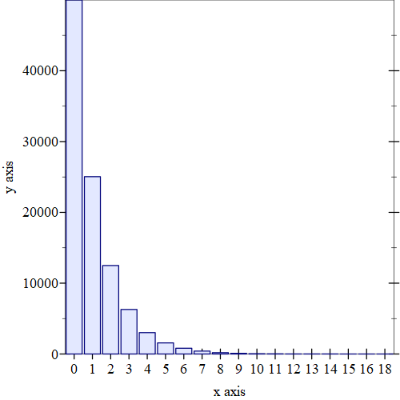
\includegraphics[width=10cm]{images/3.5.png}
    \caption{
        Histogram of geometric experiment: the \textit{x-axis} represents the values generated during the sampling phase; 
        the \textit{y-axis} represents the number of samples which have a specific value.
    }
    \label{fig:3-5}
\end{figure}


\subsection*{Exercise 3 (7)}
Convert Table~\ref{tab:es3-7} to a compact Racket program.
\begin{table}[H]
    \begin{center}
        \begin{tabular}{ccc}
            \hline
            A & B & P(A, B) \\
            \hline
            F & F & 0.14 \\
            F & T & 0.06 \\
            T & F & 0.4 \\
            T & T & 0.4 \\
            \hline
        \end{tabular}
    \end{center}
    \caption{Probabilities to be computed with a Racket program}
    \label{tab:es3-7}
\end{table}

\noindent Hint: fix the probability of A and then define the probability of B to depend on whether A is true or not. 
Run your Church program and build a histogram to check that you get the correct distribution.

\begin{lstlisting}
(define a ...)
(define b ...)
(list a b)
\end{lstlisting}

\paragraph{Solution}
The \texttt{a-b-model} has been defined as follows:
\begin{lstlisting}[caption={Model to compute the probabilities of A and B}, captionpos=b]
(define (a-b-model)
  (define a
    (flip 0.8))
  (define b
    (if a
        (flip 0.5)
        (flip 0.3)))
  (list a b))
\end{lstlisting}
The model does not contain the \texttt{rejection-sampler} because we do not need to compute a conditional probability.
The \texttt{a-b-model} defines first the variable \texttt{a} which has probability $0.8$ to be \textit{true}:
this probability can be computed by adding the last two rows of the Table~\ref{tab:es3-7}, indeed, the value of \texttt{A} in
the first two rows is \textit{false}, while in the last two is \textit{true}.
Then the probability of the variable \texttt{b} depends on the value of the variable \texttt{a}, indeed, if \texttt{A} is 
\textit{false}, then the probability that \texttt{B} is \textit{true} $ \frac{0.06}{0.06 + 0.14} = 0.3 $ (Only the rows of the table
in which \texttt{A} is \textit{false} are considered); while if \texttt{A} is \textit{true}, then the probability that \texttt{B}
is true is $ 0.5 $.

\begin{figure}[h]
    \centering
    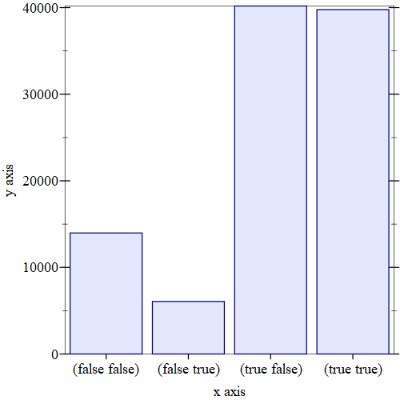
\includegraphics[width=10cm]{images/3.7.png}
    \caption{
        Histogram of A-B experiment: the \textit{x-axis} represents the values generated during the sampling phase; 
        the \textit{y-axis} represents the number of samples which have a specific value.
    }
    \label{fig:3-7}
\end{figure}

The experiment consists of generating $100000$ samples, the histogram of generated samples is shown in Figure~\ref{fig:3-7}.
It is possible to observe that the samples are distributed as the probability distribution defined in Table~\ref{tab:es3-7},
indeed, the number of samples with value false both for the variable \texttt{A} and \texttt{B} is about $14000$; the number of
samples with \texttt{A} \textit{true} is about $6000$ and the number of samples with value \textit{(true, false)} and 
\textit{(true, true)} is about $40000$ each. 
The number of samples is not exact because we are approximating the probability distribution by sampling.